\section{AP selection}\label{sec:esnr_apsel}
In a dense network, a new client may need to select its parent from many available repeaters in addition to the network coordinator. In enterprise AP and Wireless Distribution System networks today, clients typically choose the node whose probe response has the highest SNR\@. (\xxx{though there is heaps of related work doing more complex things.}) In dual-band networks, some devices may prefer a 5\GHz AP with slightly lower SNR, as long as it exceeds a minimum threshold, based on the optimistic assumption that interference is lower in the 5\GHz band. Here, we describe a procedure that uses the Effective SNR to improve this decision process and select a good parent.

Normally, a client scanning for a network cycles through the available channels sends a probe request at the lowest rate (including a single stream and 20\MHz channels), and all APs or repeaters in range respond. We propose that the client instead send multiple probes that use the lowest 6.5\Mbps rate, but vary the number of streams and channel width in decreasing order. In this way, the coordinator and all repeaters that measure CSI from the probes can compute the Effective SNR for the uplink. The probe responses can now include the computed Effective SNR to better inform the client's choice. If the client includes its transmit power level in the probe request (or if the responder makes a conservative estimate), then the responder can combine this information with the CSI measured from the probe to compute the Effective SNR for the downlink. It can then send the probe response at a faster rate than the base rate and reduce the overhead of the probe response.

%%%%%%%%%%%%%%%%%%%%%%%%%%%%%%%%%%%%%%%%%%%%%%%%
\begin{algorithm}[htp]
\caption{\label{alg:ap_sel_basic}\fcall{APSelection($A, s$)}}
\begin{algorithmic}
\STATE $t_{\max}\gets 0\Mbps$
\STATE $a_{\best} \gets \emptyset$
\FORALL{$a \in A$}
\STATE $t \gets \fcall{PredictThroughput($s, a$)}$
\IF{$t > t_{\max}$}
	\STATE $t_{\max} \gets t$
	\STATE $a_{\best} \gets a$
\ENDIF
\RETURN $a_{\best}$
\ENDFOR
\end{algorithmic}
\end{algorithm}
%%%%%%%%%%%%%%%%%%%%%%%%%%%%%%%%%%%%%%%%%%%%%%%%



\subsection{Evaluation methodology}
Compare the following strategies:
\begin{figure}[htp]
	\centering
	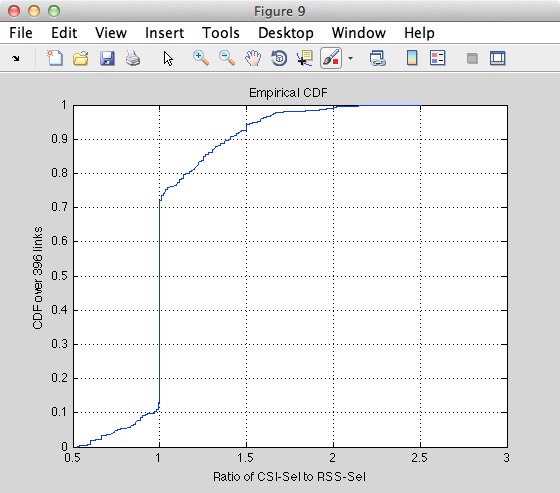
\includegraphics[width=0.6\textwidth]{figures/esnr/ap_sel_ratio.png}
	\caption{\label{fig:ap_sel_ratio}The relative throughput selecting APs by Packet SNR or by Effective SNR\@.}
\end{figure}

\begin{figure}[htp]
	\centering
	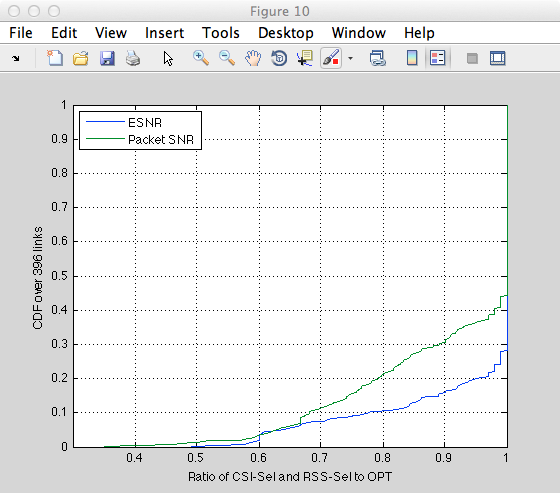
\includegraphics[width=0.6\textwidth]{figures/esnr/ap_sel_ratio_opt.png}
	\caption{\label{fig:ap_sel_ratio_opt}AP selection using Packet SNR or Effective SNR compared to Optimal.}
\end{figure}

\begin{figure}[htp]
	\centering
	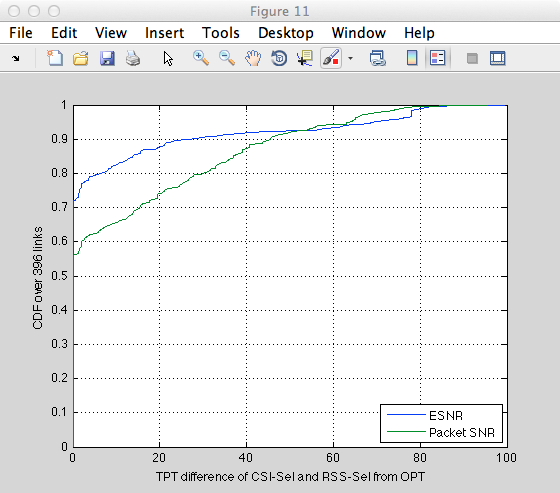
\includegraphics[width=0.6\textwidth]{figures/esnr/ap_sel_delta_opt.png}
	\caption{\label{fig:ap_sel_delta_opt}The difference in throughput using APs selected by Packet SNR or Effective SNR compared to Optimal.}
\end{figure}
\begin{itemize}
\item first AP seen
\item max RSSI
\item max CSI predicted rate
\item max measured rate
\end{itemize}